\part{Arhitektura softvera i detaljno projektovanje}

\chapter{Kratak opis}
Dokument obrađuje pregled arhitekture aplikacije \UpamtiOnline.

\chapter{Reference}
Pogledati:
\begin{enumerate}
  \item Specifikacija slučajeva korišćenja (\ref{part:use-case}) aplikacije \UpamtiOnline.
\end{enumerate}

\chapter{Reprezentacija arhitekture}
Arhitektura sistema u dokumentu je prikazana kao serija pogleda na sistem:
pogled na slučajeve upotrebe, pogled na procese, pogled na primenjeni sistem i pogled na implementaciju.
Ovi pogledi su grafički predstavljeni kao modeli pomoću jezika UML.

\chapter{Ciljevi arhitekture}

Arhitektura je dizajnirana uzimajući u obzir sledeće:
\begin{enumerate}
  \item Korisnički interfejs je pažljivo dizajniran da bi bio jednostavan i intuitivan za korišćenje.
  \item Sve akcije koje mogu dovesti u pitanje konzistentnost i validnost podataka moraju biti programski onemogućene; na primer: na istom kursu se ne mogu naći dve kartice sa identičnim pitanjem; ne sme postojati prazna lekcija ili kurs, itd.
  \item Program mora da održava vremensku konzistentnost podataka koji se unose i obrađuju, i to pomoću mehanizama koji nisu vezani za korisnika programa.
  \item Program mora da na efikasan način radi sa velikim brojem kurseva odnosno kartica koje koristnici uče.
\end{enumerate}

\chapter{Pogled na slučajeve upoterbe}
Slučajevi korišćenja mogu biti podeljeni u grupe kao što je to učinjeno u \ref{ch:use-case-uvod}.

\section{Slučajevi upotrebe značajni za arhitekturu sistema}
Slučajevi upotrebe značajni za arhitekturu sistema su \ref{subsec:ucenje}, \ref{subsec:obnavljanje} i \ref{subsec:spajalica}.

\chapter{Pogled na logičku predstavu sistema}

\section{Pregled arhitekture -- paketi, podsistemi i slojevi}

Sistem se sastoji od tri podsistema (vidi sliku \ref{fig:paketi}):
\begin{itemize}
  \item sloj podataka,
  \item logika sistema,
  \item interfejs.
\end{itemize}

\begin{figure}[htbp]
  \centering
  \begin{tikzpicture}
    \begin{umlpackage}[x=0, y=8]{korisnicki interfejs}
    \end{umlpackage}
    \begin{umlpackage}[x=0, y=4]{logika aplikacije}
    \end{umlpackage}
    \begin{umlpackage}[x=0, y=0]{sloj za prisup podacima}
    \end{umlpackage}
    \begin{umlpackage}[x=5, y=0]{baza}
    \end{umlpackage}
    \umlimport{korisnicki interfejs}{logika aplikacije}
    \umlimport{logika aplikacije}{sloj za prisup podacima}
    \umlimport{sloj za prisup podacima}{baza}
  \end{tikzpicture}
  \caption{Pregled arhitekture: paketi, podsistemi i slojevi}
  \label{fig:paketi}
\end{figure}

Sloj podataka predstavlja projekat \Filename{Data} koji služi za komunikaciju sa bazom podataka i sadrži odgovarajući API.

Logika sistema je realizovana u projektu \Filename{UpamtiMe}, koji je MVC veb-aplikacija koja se oslanja na ASP.NET frejmvork.

Interfejs sistema je realizovan kao skup HTML5 dokumenata, pisanih kao \Filename{.cshtml} pomoću Rejzorove sintakse.
Za dizajn je korišćen CSS3, generisan pomoću skript-jezika SASS i sintakse SCSS.
Za interakciju sa korisnikom, kao i asinhrono komuniciranje sa samom aplikacijom korišćen je JavaScript, i njegov frejmvork jQuery.

\chapter{Pogled na implementaciju}

\section{Baza podataka}
Slika \ref{fig:sema-baza} predstavlja bazu podataka na koju se oslanja aplikacija \UpamtiOnline.

\begin{figure}[htbp]
  \centering
  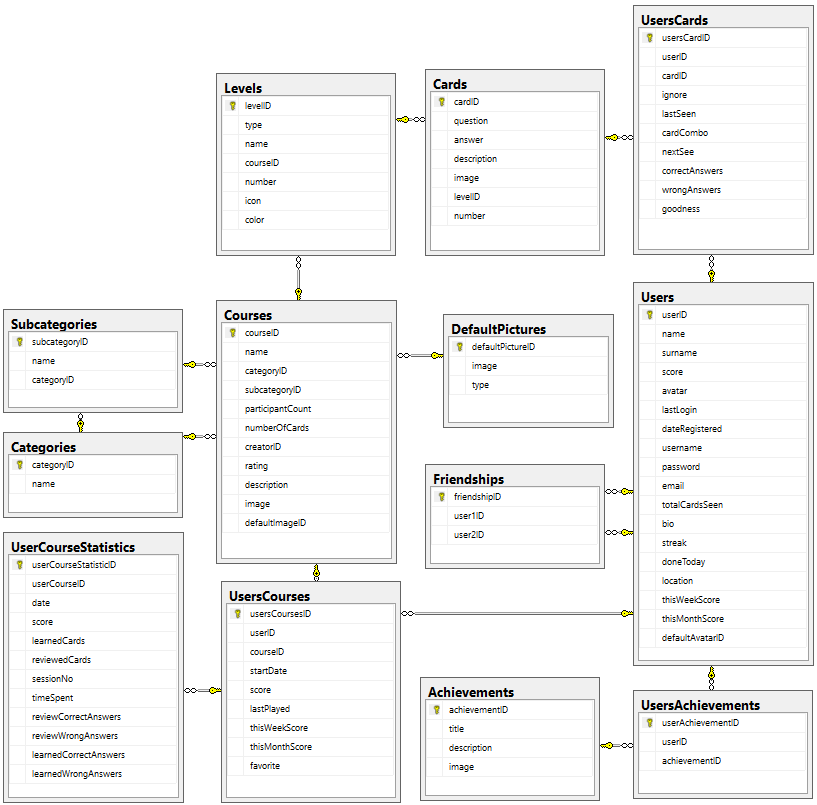
\includegraphics[scale=0.55]{baya}
  \caption{Šema baze podataka}
  \label{fig:sema-baza}
\end{figure}

\section{Sesije}
Klasni dijagram koji opisuje arhitekturu sesija prikazan je na slici \ref{fig:sesije}.

\begin{figure}
  \centering
  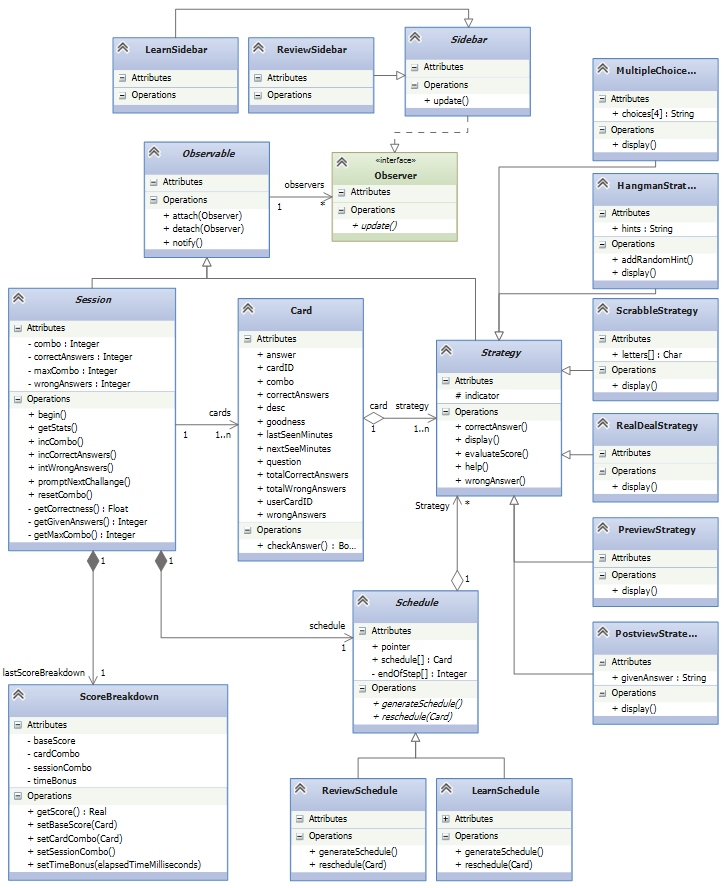
\includegraphics[scale=0.7]{yava}
  \caption{Klasni dijagram koji opisuje arhitekturu sesija}
  \label{fig:sesije}
\end{figure}

Sesija se, nezavisno od toga da li je u pitanju sesija učenja ili sesija obnavljanja, sastoji od više različitih izazova (igara).
Da bi sesija mogla da se sastoji od proizvoljnih izazova, i kako bi eventualno buduće dodavanje novih izazova u sistem bilo moguće obaviti na jednostavan način, prilikom implementacije upotrebljeni su projektni obrasci, među kojima su Unikat, Strategija i Posmatrač.

Sama sesija je implementirana kao Unikat i sadrži raspored kartica, pri čemu svaka kartica ima niz pokazivača na strategije, koje su zapravo izazovi.
Svaka strategija ima jedinstven način prikaza i neophodne podatke (na primer, izazov Hangman sadrži string u kome su samo pojedina slova prikazana).
Prilikom pokretanja sesije, na slučajan način se generiše raspored kartica, a redosled strategija svake kartice ostaje nepromenjen.

Kada korisnik tokom sesije da tačan odgovor, ta kartica prelazi na sledeću strategiju, koja će biti prikazana kada ta kartica dođe na red.
Ukoliko korisnik da netačan odgovor, strategija odgovarajuće kartice ostaje nepromenjena kako bi se ona ponovo prikazala kada sledeći put pomenuta kartica dođe na red, ali se kartica istovremeno odlaže i na kraj rasporeda.
Na taj način na pogrešeno pitanje dogovor daje više puta, kako bi se pojam urezao u korisnikovo pamćenje.
